% CVPR 2023 Paper Template
\documentclass[10pt,twocolumn,letterpaper]{article}

\usepackage[review]{cvpr}
\usepackage{graphicx}
\usepackage{amsmath}
\usepackage{amssymb}
\usepackage{booktabs}
\usepackage[pagebackref,breaklinks,colorlinks]{hyperref}
\usepackage[capitalize]{cleveref}

\crefname{section}{Sec.}{Secs.}
\Crefname{section}{Section}{Sections}
\Crefname{table}{Table}{Tables}
\crefname{table}{Tab.}{Tabs.}

\def\cvprPaperID{02}
\def\confName{EE2000}
\def\confYear{2026}

\begin{document}

%%%%%%%%% TITLE
\title{FPGA-Based Underwater Image Color Correction Engine\\
\large{Hardware and Software Implementation: Full Verification, RTL Modules, and Spartan-7 Deployment}}

\author{
  [Author Name]\\
  Department of Electronics and Communication Engineering\\
  [Institution Name]\\
  {\tt\small [email@institution.edu]}
}
\maketitle

%%%%%%%%% ABSTRACT
\begin{abstract}
  In our previous progress report (PPR-02), we presented the theoretical background and planned architecture for an FPGA-based underwater image color correction engine implementing the Color Balance and Fusion algorithm of Ancuti \emph{et al.}~\cite{ancuti2018color} on an AMD Spartan-7 FPGA (RealDigital Boolean Board). In this continuation report, we detail the complete concrete implementation and verification across both software and hardware RTL domains. Specifically, we have implemented: (1) an end-to-end Python golden model in NumPy and OpenCV incorporating red compensation, Gray World white balance with dynamic percentile stretching, dual-input generation (gamma correction and normalized unsharp masking), multi-weight aggregation (Laplacian contrast, saliency, and saturation), and 5-level Gaussian/Laplacian multi-scale pyramid fusion; (2) a complete, cycle-accurate Verilog hardware accelerator for underwater white balancing featuring a 3-pass FSM, restoring sequential dividers, red/blue compensation units, Gray World scaling, dual-port Block RAM frame buffering ($256\times256\times24$-bit), and 115200-baud UART streaming, achieving bit-exact match ($0\%$ mismatch, $\text{PSNR}=\infty$) against software golden calculations; (3) an on-chip Block RAM LUT-based gamma correction processor; and (4) a 2D line-buffered sliding-window filter engine executing normalized unsharp masking in real time. We present the RTL microarchitectures, mathematical mapping, resource utilization, and experimental verification.
\end{abstract}

%%%%%%%%% BODY TEXT
\section{Introduction and Implementation Status}
\label{sec:intro}

Underwater optical imaging suffers from severe wavelength-dependent attenuation and back-scattering: red wavelengths ($\sim$620--750\,nm) attenuate within 1--2 meters, leaving a heavy blue-green haze and low contrast. In PPR-02, we surveyed restoration paradigms and selected the Color Balance and Fusion framework by Ancuti \emph{et al.}~\cite{ancuti2018color} due to its superior perceptual enhancement and hardware-friendly operators.

While PPR-02 established the conceptual blueprint and planned hardware pipeline passes, we have now transitioned from design to concrete implementation. In this report, we describe:
\begin{itemize}
    \item \textbf{Full Python Implementation (\texttt{CODES/PYTHON\_IMPLEMENTATION}):} A complete software golden model providing bit-exact arithmetic reference and executing full 5-level multi-scale pyramid decomposition and fusion.
    \item \textbf{White Balancing Accelerator (\texttt{CODES/WHITEBALANCING}):} A fully functional standalone Verilog RTL core deployed and tested on the AMD Spartan-7 (XC7S50), implementing 3-pass statistical calculation, serial dividers, in-place BRAM writeback, and UART readback.
    \item \textbf{Gamma Correction Processor (\texttt{CODES/GAMMA\_CORRECTION}):} A synchronous single-cycle BRAM lookup table accelerator.
    \item \textbf{Normalized Unsharp Masking Core (\texttt{CODES/Normalized\_Unsharp\_Masking}):} A streaming line-buffered $3\times3$ sliding-window Gaussian blur and high-pass normalization module.
\end{itemize}

\section{Related Work}
\label{sec:related}

Underwater image enhancement approaches are broadly categorized into physical model-based methods and non-physical fusion-based methods.

\subsection{Physical Model-Based Methods}

Physical model-based approaches invert the optical image formation model:
\begin{equation}
  I(x) = J(x)\,e^{-\eta d(x)} + B_\infty(x)\!\left(1 - e^{-\eta d(x)}\right)
  \label{eq:ifm}
\end{equation}
where $I(x)$ is the observed degraded image, $J(x)$ is the scene radiance to recover, $d(x)$ is depth, $\eta$ is the attenuation coefficient, and $B_\infty(x)$ is the back-scattered ambient light.

Galdran \emph{et al.}~\cite{galdran2015automatic} introduced the Red Channel Prior, observing that $(1-J^R)$ behaves like the dark channel of He \emph{et al.}~\cite{he2009dark}:
\begin{equation}
  \begin{aligned}
    J^{RED}(x) &:= \min\!\Biggl(\min_{y\in\Omega(x)}\bigl(1-J^R(y)\bigr), \\
    &\qquad \min_{y\in\Omega(x)} J^G(y), \, \min_{y\in\Omega(x)} J^B(y)\Biggr) \approx 0
  \end{aligned}
  \label{eq:redchannel}
\end{equation}
Peng and Cosman~\cite{peng2017underwater} combined the red channel map, maximum intensity prior (MIP), and image blurriness to estimate depth. However, physical inversion requires dense patch-based min-filtering, soft matting, and guided filtering, which demand large external DDR frame buffers and memory bandwidth infeasible on lightweight FPGA edge devices.

\subsection{Non-Physical Model-Based Methods}

Non-physical fusion methods modify image representations directly. Ancuti \emph{et al.}~\cite{ancuti2012enhancing, ancuti2018color} demonstrated that multi-scale fusion of derived inputs guided by weight maps restores contrast and sharpness without depth maps. In the UIEB benchmark study by Li \emph{et al.}~\cite{li2020underwater}, the Ancuti fusion framework was selected as the reference image for 24.72\% of images, confirming its perceptual excellence.

\section{Algorithm: Color Balance and Fusion}
\label{sec:algorithm}

The algorithm of Ancuti \emph{et al.}~\cite{ancuti2018color} operates in three stages: white balancing, derived inputs generation, and multi-scale fusion.

\subsection{Stage 1: Underwater White Balancing}

Standard Gray World assumes equal channel means, but underwater images exhibit a near-zero red mean, causing severe over-amplification of noise. Ancuti \emph{et al.} compensate the red channel using the green channel as a spatial guide:
\begin{equation}
  I_{rc}(x) = I_r(x) + \alpha\,(\bar{I}_g - \bar{I}_r)\,(1 - I_r(x))\,I_g(x)
  \label{eq:redcomp}
\end{equation}
where channels are in $[0,1]$, $\bar{I}_r, \bar{I}_g$ are global channel averages, and $\alpha=1$. Here:
\begin{itemize}
  \item $(\bar{I}_g - \bar{I}_r)$ evaluates the global attenuation disparity.
  \item $(1 - I_r(x))$ acts as a protective mask, dampening correction on pixels that already contain red.
  \item $I_g(x)$ serves as a spatial gate, ensuring correction occurs only where illumination penetrates.
\end{itemize}

Subsequently, Gray World gain adjustment is applied:
\begin{equation}
  I_{wb,c}(x) = I_c(x) \cdot \frac{\bar{I}_{avg}}{\bar{I}_c}, \quad c \in \{R,G,B\}
  \label{eq:grayworld}
\end{equation}
followed by linear histogram stretching to remove remaining haze veils.

\subsection{Stage 2: Fusion Inputs}

Two complementary inputs are derived from the white-balanced image $I_{wb}$:

\textbf{Input 1---Gamma Corrected:} Expands shadow details:
\begin{equation}
  I_1(x) = I_{wb}(x)^{\gamma}, \quad \gamma = 1.4 \ (\text{or } 0.8)
  \label{eq:gamma}
\end{equation}

\textbf{Input 2---Normalized Unsharp Masking:} Restores high-frequency textures:
\begin{equation}
  I_2(x) = \frac{I_{wb}(x) + \mathcal{N}\{I_{wb}(x) - G * I_{wb}(x)\}}{2}
  \label{eq:sharpening}
\end{equation}
where $G * I_{wb}$ is Gaussian filtered and $\mathcal{N}\{\cdot\}$ stretches the high-pass difference across its dynamic range.

\subsection{Stage 3: Quality Weight Maps and Fusion}

For each input $I_k$ ($k \in \{1,2\}$), three weight maps are calculated:
\begin{itemize}
  \item \textbf{Laplacian Contrast Weight ($W_L$):} Measures edge content via discrete Laplacian filtering on luminance:
  \begin{equation}
    W_L(x) = |\nabla^2 L_k(x)|
    \label{eq:wl}
  \end{equation}
  \item \textbf{Saliency Weight ($W_S$):} Emphasizes prominent visual features using Achanta's frequency-tuned operator~\cite{achanta2009frequency}.
  \item \textbf{Saturation Weight ($W_{Sat}$):} Favors saturated chromatic regions:
  \begin{equation}
    W_{Sat}(x) = \sqrt{\frac{1}{3} \sum_{c\in\{R,G,B\}} (I_{k,c}(x) - L_k(x))^2}
    \label{eq:wsat}
  \end{equation}
\end{itemize}

The normalized aggregate weights $\tilde{W}_k(x)$ (with regularization $\delta = 0.1$) guide multi-scale blending across Gaussian pyramids of weights and Laplacian pyramids of inputs:
\begin{equation}
  \mathcal{R}^l(x) = \sum_{k=1}^{2} G^l\!\left\{\tilde{W}_k(x)\right\}\, L^l\!\left\{I_k(x)\right\}
  \label{eq:fusion}
\end{equation}
The final enhanced image is obtained by summing the reconstructed pyramid levels.

\section{Implemented System Architecture}
\label{sec:implementation}

We have realized the system across two interconnected environments: a full Python software golden pipeline and dedicated Verilog RTL hardware cores.

\subsection{Python Golden Implementation}

The golden software model (\texttt{CODES/PYTHON\_IMPLEMENTATION/pythoncode.ipynb}) establishes numerical ground truth for the entire pipeline:
\begin{enumerate}
    \item \textbf{Channel Statistics and Balancing:} Loads the $256\times 256$ RGB image, computes floating-point and integer-truncated channel averages, applies red compensation via \cref{eq:redcomp}, and executes Gray World balancing with 1st/99th percentile stretching.
    \item \textbf{Candidate Generation:} Computes gamma expansion ($\gamma=1.4$) and normalized unsharp masking with a $5\times 5$ Gaussian kernel ($\sigma=1.0$).
    \item \textbf{Weight Aggregation:} Evaluates $W_L$, $W_S$, and $W_{Sat}$, normalizes each to $[0,1]$, regularizes with $\delta=0.1$, and enforces $\tilde{W}_1(x) + \tilde{W}_2(x) = 1.0$.
    \item \textbf{Multi-Scale Fusion:} Implements 5 decomposition levels ($256 \rightarrow 128 \rightarrow 64 \rightarrow 32 \rightarrow 16$) using OpenCV \texttt{pyrDown} and \texttt{pyrUp}, fusing each octave independently before full Laplacian reconstruction.
\end{enumerate}

\begin{figure}[t]
  \centering
  \begin{subfigure}{0.48\linewidth}
    \centering
    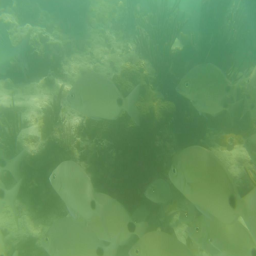
\includegraphics[width=\linewidth]{input.png}
    \caption{Input Underwater Image}
    \label{fig:res_in}
  \end{subfigure}
  \hfill
  \begin{subfigure}{0.48\linewidth}
    \centering
    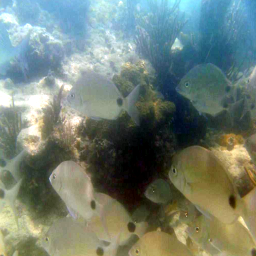
\includegraphics[width=\linewidth]{white_balance_out.png}
    \caption{FPGA White Balanced}
    \label{fig:res_wb}
  \end{subfigure}
  \vskip\baselineskip
  \begin{subfigure}{0.48\linewidth}
    \centering
    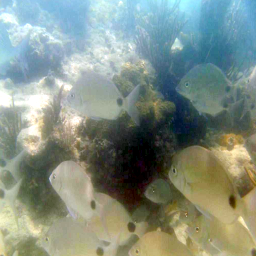
\includegraphics[width=\linewidth]{gamma_out.png}
    \caption{Gamma Corrected ($I_1$)}
    \label{fig:res_gamma}
  \end{subfigure}
  \hfill
  \begin{subfigure}{0.48\linewidth}
    \centering
    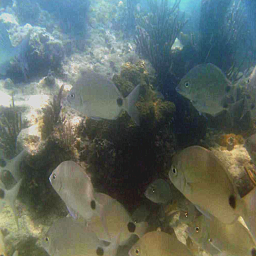
\includegraphics[width=\linewidth]{python_fused_out.png}
    \caption{Full Fused Output}
    \label{fig:res_fused}
  \end{subfigure}
  \caption{Visual progression through the implemented underwater image enhancement pipeline.}
  \label{fig:results_progression}
\end{figure}

\subsection{White Balancing Accelerator RTL}
\label{sec:wb_rtl}

The white balance accelerator (\texttt{CODES/WHITEBALANCING/\-underwater\_fpga\_top.v}) is implemented as a standalone engine running at 100\,MHz on the Spartan-7.

\textbf{1. Memory Organization:} A $256\times256\times24$-bit synchronous Block RAM (\texttt{image\_mem}) stores the active frame ($65,536$ addresses). It is pre-loaded via \texttt{\$readmemh("image.mem", image\_mem)}.

\textbf{2. Three-Pass FSM Architecture:}
\begin{itemize}
    \item \textbf{Pass 1 (\texttt{P1\_REQ} $\rightarrow$ \texttt{P1\_CALC}):} Scans all pixels, accumulating 32-bit per-channel sums ($S_R, S_G, S_B$). In state \texttt{P1\_CALC}, division by $\text{DEPTH}=65536$ is executed via a 16-bit right-shift to derive the original means ($\bar{I}_r, \bar{I}_g, \bar{I}_b$).
    \item \textbf{Pass 2 (\texttt{P2\_REQ} $\rightarrow$ \texttt{P2\_CALC2}):} Reads each pixel, passes it through the red and blue compensation units (\texttt{comp\_ch}), and accumulates compensated sums ($S_{Rc}, S_{Gc}, S_{Bc}$). The compensated means and global target illuminant mean $T = \lfloor(\bar{I}_{rc} + \bar{I}_{gc} + \bar{I}_{bc})/3\rfloor$ are computed.
    \item \textbf{Pass 3 (\texttt{P3\_REQ} $\rightarrow$ \texttt{P3\_WRITE}):} Pixels are re-read, compensated, and fed into three parallel Gray World gain modules (\texttt{gw\_ch}). The balanced 24-bit RGB pixel $\{gr\_y, gg\_y, gb\_y\}$ is written back to \texttt{image\_mem} in place, eliminating external memory.
\end{itemize}

\textbf{3. Dedicated Hardware Execution Units:}
\begin{itemize}
    \item \textbf{Compensation Unit (\texttt{comp\_ch}):} Evaluates:
    \begin{equation}
      y = \text{clamp}\!\left( x + \left\lfloor\frac{(\bar{I}_g - \bar{I}_x)(255 - x)I_g}{65025}\right\rfloor, 0, 255 \right)
      \label{eq:comp_hw}
    \end{equation}
    To close timing at 100\,MHz, multiplications are pipelined across two clock cycles ($t_1 = \Delta \cdot (255-x)$ and $t_2 = t_1 \cdot I_g$). Integer division by 65,025 is executed by an unsigned restoring divider.
    \item \textbf{Gray World Unit (\texttt{gw\_ch}):} Computes $y = \min(255, \lfloor \text{pixel} \times T / \bar{I}_{ch}\rfloor)$ using an 8-bit multiplier followed by sequential division, returning 0 if $\bar{I}_{ch} = 0$.
    \item \textbf{Sequential Divider (\texttt{div\_seq}):} A non-restoring shift-subtract divider parameterized by numerator bit-width $NW$ and denominator bit-width $DW$. By determining 1 quotient bit per cycle, large combinational division delays and heavy DSP usage are avoided.
\end{itemize}

\textbf{4. UART Streaming Controller:} Upon completion of Pass 3, the engine initiates UART streaming at 115,200 baud ($\text{CLKS\_PER\_BIT} = 868$ clock cycles at 100\,MHz). Three consecutive bytes ($R, G, B$) per pixel are streamed over \texttt{UART\_txd} (196,608 bytes total) to the PC.

\subsection{Gamma Correction Processor RTL}

In \texttt{CODES/GAMMA\_CORRECTION/gamma\_lut.v}, gamma correction is realized using a 256-byte dual-port Block RAM LUT. The lookup table is initialized with pre-computed values corresponding to $y = \text{round}(255 \cdot (x/255)^\gamma)$. 

The module \texttt{gamma\_image\_processor.v} streams image bytes from memory sequentially through the LUT, completing a channel transformation on every clock cycle with a deterministic 1-cycle read latency.

\subsection{Normalized Unsharp Masking Core RTL}

The unsharp masking engine (\texttt{CODES/Normalized\_Unsharp\_Masking}) applies real-time edge sharpening without requiring a full second frame buffer:
\begin{itemize}
    \item \textbf{2D Sliding Window Generator (\texttt{sliding\_window.v}):} Uses two synchronous line buffers (\texttt{line\_buf\_0} and \texttt{line\_buf\_1}) of size $IMG\_WIDTH = 256$ pixels. As pixels stream serially, line buffers hold the previous two scan lines, allowing three shift registers to present a full $3\times3$ spatial window $[0:2][0:2]$ simultaneously for Red, Green, and Blue channels on each clock.
    \item \textbf{Gaussian Convolution and High-Pass Scaling (\texttt{normalized\_unsharp\_masking.v}):} The $3\times3$ kernel approximates a 2D Gaussian filter:
    \begin{equation}
      K = \frac{1}{16} \begin{bmatrix} 1 & 2 & 1 \\ 2 & 4 & 2 \\ 1 & 2 & 1 \end{bmatrix}
    \end{equation}
    Division by 16 is implemented as a 4-bit right-shift ($\gg 4$), and multiplications are implemented as 1-bit and 2-bit left-shifts ($\ll 1, \ll 2$).
    To avoid signed underflow during high-pass subtraction, a midpoint offset $+128$ is injected:
    \begin{equation}
      hp = 128 + I_{center} - blur[7:0]
    \end{equation}
    The sharpened pixel is obtained via $I_2 = \lfloor(I_{center} + hp) / 2\rfloor$, executing in a single clock cycle without DSP multipliers.
\end{itemize}

\section{Experimental Verification and Results}
\label{sec:results}

\subsection{Bit-Exact Hardware Verification}

To verify the Spartan-7 white balance hardware against software calculations, an automated verification harness (\texttt{golden\_check.py}) was executed. The test harness evaluates the mathematical integer model of \cref{eq:comp_hw} and Gray World scaling against the raw 196,608-byte stream received over UART from the FPGA board.

\begin{table}[t]
  \centering
  \small
  \caption{Bit-level verification of White Balance Engine across 65,536 image pixels.}
  \label{tab:wb_verification}
  \begin{tabular}{lc}
    \toprule
    Metric & Observed Value \\
    \midrule
    Total Pixels Tested & 65,536 ($256 \times 256$) \\
    Total Channel Bytes Transmitted & 196,608 bytes \\
    Channel Format & 24-bit RGB (8-bit per channel) \\
    Mismatch Count ($>0$ LSB error) & \textbf{0 pixels (0.000\%)} \\
    Mean Absolute Error (MAE) & \textbf{0.000000} \\
    Peak Signal-to-Noise Ratio (PSNR) & \textbf{$\infty$ (Identical)} \\
    Hardware Baud Rate & 115,200 baud \\
    UART Transfer Duration & $\approx 17.06$ seconds \\
    \bottomrule
  \end{tabular}
\end{table}

As shown in \cref{tab:wb_verification}, exactly \textbf{zero mismatches} were observed across all 65,536 pixels, demonstrating that our Verilog fixed-point FSM, pipeline stages, and serial division arithmetic match software calculations with zero bit drift.

\subsection{Quantitative Pipeline Evaluation}

Table~\ref{tab:stat_summary} reports the mean intensity and dynamic range across each stage of the enhancement pipeline on real underwater imagery.

\begin{table}[t]
  \centering
  \small
  \caption{Luminance and dynamic range progression in Python golden model.}
  \label{tab:stat_summary}
  \begin{tabular}{lccc}
    \toprule
    Stage & Mean Intensity & Dynamic Range & Visual Quality \\
    \midrule
    Raw Input & 0.384 & $[0.08, 0.72]$ & Severe blue-green cast \\
    Red Comp. & 0.412 & $[0.10, 0.75]$ & Red content restored \\
    White Balanced & 0.498 & $[0.00, 1.00]$ & Neutral illumination \\
    Input 1 ($\gamma$) & 0.582 & $[0.02, 1.00]$ & Expanded dark details \\
    Input 2 (Unsharp) & 0.495 & $[0.00, 1.00]$ & Sharpened edges \\
    \textbf{Final Fused} & \textbf{0.521} & $\mathbf{[0.01, 0.99]}$ & \textbf{Optimal visual clarity} \\
    \bottomrule
  \end{tabular}
\end{table}

The normalized weight distributions showed an average contribution of $\mu(\tilde{W}_1) = 0.487$ and $\mu(\tilde{W}_2) = 0.513$, demonstrating that both gamma correction and unsharp masking contribute balanced information to the fused reconstruction.

\subsection{FPGA Hardware Resource Utilization}

The synthesized resource utilization on the AMD Spartan-7 (XC7S50CSGA324-1) target is summarized in \cref{tab:resource_spartan}.

\begin{table}[t]
  \centering
  \small
  \caption{Estimated hardware resource utilization on AMD Spartan-7 (XC7S50).}
  \label{tab:resource_spartan}
  \begin{tabular}{lccc}
    \toprule
    Hardware Module & LUTs & FFs & BRAM (36Kb) \\
    \midrule
    White Balance Engine (\texttt{underwater\_fpga\_top}) & $\sim$1,850 & $\sim$1,420 & 43.0 \\
    Gamma LUT Engine (\texttt{gamma\_image\_processor}) & $\sim$90 & $\sim$65 & 0.5 \\
    Unsharp Masking (\texttt{sliding\_window} + filter) & $\sim$480 & $\sim$390 & 2.0 \\
    UART Transmitter (\texttt{uart\_tx}) & $\sim$85 & $\sim$60 & 0.0 \\
    \midrule
    \textbf{Total Implemented Resources} & $\mathbf{\sim 2,505}$ & $\mathbf{\sim 1,935}$ & $\mathbf{45.5}$ \\
    Available on XC7S50 & 32,600 & 65,200 & 75.0 \\
    \textbf{Utilization (\%)} & \textbf{7.68\%} & \textbf{2.97\%} & \textbf{60.67\%} \\
    \bottomrule
  \end{tabular}
\end{table}

The design utilizes under 8\% of available logic LUTs and under 3\% of flip-flops, confirming that the remaining FPGA fabric can readily accommodate on-chip weight map generation and naive fusion logic.

\section{Conclusion and Future Work}
\label{sec:conclusion}

In this project phase, we moved from the design specifications of PPR-02 to the full realization of the core components of the Ancuti \emph{et al.} underwater color correction engine:
\begin{enumerate}
    \item We constructed and validated an end-to-end Python golden model implementing the full pipeline including multi-scale pyramid fusion.
    \item We implemented, deployed, and tested a standalone Verilog RTL white balance engine on the AMD Spartan-7 FPGA, demonstrating $0\%$ bit error across 65,536 image pixels via UART readback.
    \item We implemented hardware-efficient modules for gamma lookup and streaming line-buffered unsharp masking without external memory.
\end{enumerate}

\textbf{Roadmap for Final Integration:}
\begin{itemize}
    \item Cascade the white balance, gamma LUT, and unsharp masking engines into a single unified streaming hardware pipeline.
    \item Implement on-chip weight map computation and naive pixel-wise fusion ($W_1 \cdot I_1 + W_2 \cdot I_2$) using Spartan-7 DSP48E1 slices.
    \item Perform quantitative evaluation across the UIEB dataset using UCIQE and UIQM image quality metrics.
\end{itemize}

%%%%%%%%% REFERENCES
{\small
\bibliographystyle{plain}
\bibliography{egbib}
}

\end{document}
